\documentclass[11pt, oneside, titlepage]{article}  
\usepackage[lmargin=1in,rmargin=1in,tmargin=1in,bmargin=1in]{geometry}
\geometry{letterpaper}

\usepackage{indentfirst} % INDENTS FIRST PARAGRAPH
\usepackage{graphicx}
\usepackage{amssymb} 
\usepackage{amsmath} % better math stuff
\usepackage{multicol} % columns in text
\usepackage{enumitem} % less space between bullets

% ALLOWS FOR HYPERLINKS
\usepackage{hyperref}
\hypersetup{hidelinks}      


% TABLE OF CONTENTS
\renewcommand*\contentsname{TABLE OF CONTENTS}
%\setcounter{tocdepth}{2}


% HEADERS & FOOTERS & COLORS
\usepackage{fancyhdr}
\usepackage{etoolbox,fancyhdr,xcolor}
\newcommand{\headrulecolor}[1]{\patchcmd{\headrule}{\hrule}{\color{#1}\hrule}{}{}} %ALLOW COLOR CHANGE
\newcommand{\footrulecolor}[1]{\patchcmd{\footrule}{\hrule}{\color{#1}\hrule}{}{}} %ALLOW COLOR CHANGE
\pagestyle{fancy}
\fancyhf{}% Clear header/footer
\renewcommand{\headrulewidth}{2pt}% Default \headrulewidth is 0.4pt
\renewcommand{\footrulewidth}{0.5pt}% Default \footrulewidth is 0pt
\headrulecolor{red!70}% Set header rule colour to 70% red.
\fancyfoot[R]{Page \thepage} % PAGE NUMBER
\fancyhead[R]{
\includegraphics[height=0.8cm]{graphics/mcgill_header.jpeg}} % MCGILL LOGO


% SECTION COLORS
\usepackage{xcolor}
\usepackage{sectsty}
\sectionfont{\color{red!70}}


% TITLE PAGE
\usepackage{pdfpages}
\title{MGSC-662-075 - Decision Analytics \\ 
    Routing Problem}
\author{Emery Dittmer - 260658030\\ 
    Ben Meiga - 260866790 \\ 
    Lucie Peccoux - 261087296 \\ 
    Konstantin Volodin - 261083570}
%\date{}							% Activate to display a given date or no date


% BIBLIOGRAPHY
\usepackage[backend=biber, style=chem-acs]{biblatex}
\addbibresource{bib.bib} %Import the bibliography file


%%%%% BEGIN DOCUMENT
\begin{document}
\renewcommand\refname{REFERENCES} 
\baselineskip=15pt
%\maketitle
\begin{minipage}{\textwidth}
    
\includepdf{graphics/firstpage}
\end{minipage}
\newpage

\tableofcontents
\thispagestyle{empty} % PREVENTS NUMBERING
\clearpage\setcounter{page}{1} % Start including page numbers from here

%%%%% INTRODUCTION
\newpage
%%%%%%%%%%%%%%%%
%%% Introduction
%%%%%%%%%%%%%%%%
\section*{INTRODUCTION}
\addcontentsline{toc}{section}{INTRODUCTION}



\indent Fire burns. Wind blows. Humans have mastered fire, but not its consequences. Fire creates CO2, a major contributor to greenhouse gas emissions that permanently alters our environment. Electricity generation from coal and natural gas is a major global contributor to annual CO2 emissions. The pursuit of net zero emissions by 2050 is a continuous challenge \cite{RN19}. Over the last 3 decades, wind turbines have appeared as a leading source of clean, reliable, and renewable electricity generation. More wind farms are being commissioned at an increasing rate. Engineers have begun to master the wind with larger, more efficient, and cheaper turbines \cite{RN18}. As time moves forward net zero emissions in the next thirty years seems an achievable goal. However, wind turbines have a dirty little secret: replaced blades. The wind turbine blades are progressively degraded by the environment and crucially dust \cite{RN1}. At the end of their 20-year lifespan, they need replacing. Most wind turbine blades are made from lightweight and strong fiberglass composites that are difficult to recycle. So, most old blades are buried or left in the fields. The blades eventually degrade contaminating groundwater and soil. We should not have to trade off greenhouse gas emissions and environmental degradation. Therefore, we must recycle the blades to preserve the environment. 

There is good news as engineers have developed ways of recycling fiberglass blades at specialized facilities \cite{RN3}. However, the location of these facilities remains a challenging subject. This is where data scientists can help. Optimizing the locations of facilities is a data challenge. Specifically, we must balance high capital costs for specialized equipment and long-term transportation costs between wind farms and facilities. There may be many optimal solutions or formulations. For instance, is it more cost-effective to build 20 facilities to reduce shipping costs or only 1 facility with increased shipping costs but low capital costs? Further increasing the complexity, the facilities must maintain enough supply of discarded blades to continue working or risk standing idle. Wind farms will replace all the blades at once creating a lumpy supply that creates additional challenges. We will model and address these constraints through data science and the art of optimization. 

We will examine the wind turbine industry of Ontario, considering a planning horizon of 50 years. Ontario produces around 40\% of all wind energy in Canada \cite{RN10}.  Therefore, Ontario has sufficiently diverse wind farm locations and a large enough dataset to fully model the complexity of the problem. The challenge, here, is to perfect the locations for these facilities within Ontario such that costs are minimized while ensuring a sufficient continuous supply of blades for processing. To push the problem further we will investigate a travelling salesman-style problem, involving specialized blade-cutting machinery. This equipment must travel to the wind turbines to cut them up for easier transportation. The recycling costs are associated with the cutting, transportation, storage, and disposal of the blades. Wind turbine blades have a lifetime of 20 years \cite{RN2}.

%%%%% PROBLEM DESCRIPTION
%%%%%%%%%%%%%%%%
%%% PROBLEM DESCRIPTION
%%%%%%%%%%%%%%%%
\section{PROBLEM DESCRIPTION AND FORMULATION}
\label{section:problem_desc}




\subsection{Problem Description \& Scope}
Location optimization problems balance distances with a series of weights to meet the objective function. We will be using a specific type of localization formulation: the Capacitated Multi-Facility Weber Problem (CMFWP) \cite{RN4}. This approach reduces computational power while minimizing transportation and fixed costs. The optimal solution will satisfy discarded blade supply within Ontario by placing facilities in a Euclidean plane and solving the problem in a 2 steps approach. The supply and location of each wind farm are known while the transportation cost between wind farms and facilities are proportional to their Manhattan distance. 

Separately we will look at a "routing problem" based on the travelling salesman method. The idea is to minimize the number and cost of specialized trucks that travel between wind farms to cut the discarded blades into smaller pieces for easier transportation. This is an important step for efficient turbine recycling. 

For simplicity, we will use a long-term approach, as it stabilizes both the supply and capacity of turbine blades. Both problems are limited to Ontario which has a complex network of 108 wind farms. 


%%%%%%%%%%%%%%%%
%%% MODEL ASSUMPTION
%%%%%%%%%%%%%%%%
\subsection{Model Assumptions}
Assumptions were needed to model these problems, which are described in the paragraphs below. 

\subsubsection{Transportation}
\begin{itemize}[noitemsep]
  \item We assume that we are renting transportation trucks for delivery. This implies only-way transportation. 
  \item Ontario's cost of transportation is \$47.5/mile \$29.5/km \cite{RN5}.  
  \item Transport does not have to be full, and the number of trucks required is rounded up.  For example, in a case where 3.5 trucks are needed, we’ll use 4 trucks. The optimal loading of the trucks is out of scope. 
  \item We will use Manhattan distance as many rural highways are straight North-South or East-West. 
  \item Transport trucks have a max load weight of 62.5 tonnes on Canadian Roads \cite{RN6}.
\end{itemize}

\subsubsection{Waste Details}
\begin{itemize}[noitemsep]
  \item Based on our research, we estimate the weight of one blade to be 36 tonnes \cite{RN7} \cite{RN8}.
  \item We assume that all the wind turbines are the same, I.e., the newest generation. 
  \item Each wind turbine is made of 3 blades (standard).  
  \item The blades have an average life of 20 years.
\end{itemize}

\subsubsection{Facilities}
\begin{itemize}[noitemsep]
    \item Fixed cost is based on a per tonne capacity and economies of scale with 3 types of facilities \cite{RN9} \cite{RN13}
    \begin{itemize}[noitemsep]
        \item Small: 3,000 tonnes capacity \$3.3 million 
        \item Medium: 4,500 tonnes capacity \$4.62 million (estimate) 
        \item Large capacity: 6,000 tonnes capacity \$5.94 million (estimate) 
    \end{itemize}
    \item Facilities can be placed anywhere except cities and water.  
    \item Based on the assumption stated above, we will not need to worry about negotiating land.
\end{itemize}    
\subsubsection{Cutting Trucks}
\begin{itemize}[noitemsep]
  \item Based on the waste assumption and calculation, we assume that we need to cut 400 blades per year. 
  \begin{itemize}[noitemsep]
      \item
      Total number of turbines in the province * 5\% yearly waste * 3 blades per turbine. 
  \end{itemize} 
  \item The annual capacity of cutting trucks is 300 blades, based on estimates. No official value was found.
  \item Travel cost for cutting trucks is estimated at \$29.5/km of distance travel. 
\end{itemize}

\subsection{Model Limitations}
\begin{itemize}[noitemsep]
  \item We focus on Ontario for this study as it accounts for 40\% of total wind energy production in Canada. 
  \item Each province will have different legislation and subsidies around the facility locations. 
  \item We assume that the storage of blades is not in scope. Therefore, waste storage has no cost. 
  \item There will be no significant long-term changes to the number of wind farms. This allows us to estimate the waste of wind farms as a constant. Every year 5\% of the wind farms’ blades need to be replaced. 
  \item We assume that each longitude and latitude degree is approximately 111 kilometers (about 68.97 mi).  
  \item We Look at a 50-year timeframe 
  \begin{itemize}[noitemsep]
    \item The 50 years period smooths the lumpy supply for a pseudo-steady state supply and demand. 
    \item It helps to balance the cost of transportation and the cost of site construction. 
    \item We multiply the transportation cost by 50 to ensure it considers the 50 years period.
  \end{itemize}
\end{itemize}



%%%%%%%%%%%%%%%%
%%% RECYCLING FACILITIES LOCATION PROBLEM
%%%%%%%%%%%%%%%%
\subsection{Recycling Facilities Location Problem }
\subsubsection{Model Formulation}
We solve this model in a two-stage approach to simplify the computational demands. Each stage contains generic model components and components only relevant to the stage.
\begin{enumerate}[noitemsep]
   \item Assign the entire supply of each wind turbine to a specific facility. 
   \item  Enforce the location of each facility and redistribute wind farm supply.
\end{enumerate}


%%% SETS
\subsubsection{Sets}
\begin{itemize} [noitemsep]
    \item $W$ - wind farm
    \item $T$ - facility type
    \item $F$ - facility count $ \in \{1,2...,10 \} $
\end{itemize}


%%% DATA PARAMETERS
\newpage
\subsubsection{Data Requirements}
\begin{multicols}{2}
\begin{itemize} [noitemsep]
    \item $wx_{w}$ - longitude of wind farm $w$
    \item $wy_{w}$ - latitude of wind farm $w$
    \item $wd_{w}$ - yearly deliveries from wind farm $w$
    \item $ww_{w}$ - yearly waste per delivery from $w$

    \item $co_{t}$ - building cost of facility of type $t$
    \item $ca_{t}$ - capacity of facility of type $t$

    \item $dc$ - delivery cost per truck per km
    \item $ph$ - planning horizon (years)
    \item $dk$ - conversion of latitude/longitude to km
\end{itemize}
\end{multicols}


%%% Decision Variables
\subsubsection{Decision Variables}
\begin{itemize} [noitemsep]
    \item $fb_{ft}$ - binary indicating whether facility number $f$ of type $t$ should be built
    \item $fx_{ft}$ - continuous indicating longitude of facility number $f$ of type $t$
    \item $fy_{ft}$ - continuous indicating latitude of facility number $f$ of type $t$ 

    \item $dist\_x_{wft}$ - continuous indicating longitude distance between wind farm $w$, facility $f$ of type $t$
    \item $dist\_y_{wft}$ - continuous indicating latitude distance between wind farm $w$, facility $f$ of type  $t$
    \item $dist_{wft}$ - continuous  indicating manhattan distance between wind farm $w$, facility $f$ of type $t$ 
\end{itemize}
\textbf{Stage 1:} $wa_{wft}$ - binary variable assigning wind farm $w$ to facility $f,t$ \\ 
\textbf{Stage 2:} $dw_{wft}$ - integer variable indicating how many deliveries to make from $w$ to $f,t$


%%% Constraints
\subsubsection{Constraints}
Demand
\vspace{-5pt}
\begin{equation}
\begin{aligned}
	\sum_{t,f} wa_{wft} 	& = & 1  		& \quad \forall w \quad \quad 	& \text{Stage 1} \\ 
	\sum_{t,f} dw_{wft} 	& = & wd_{w}  	& \quad \forall w \quad \quad 	& \text{Stage 2}
\end{aligned}
\end{equation}

Capacity
\vspace{-5pt}
\begin{equation}
\begin{aligned}
	\sum_{t,f} wa_{wft} * ww_{w} * wd_{w} 	& \le & ca_{t} * fb_{ft}		& \quad \forall w  \quad  	& \text{Stage 1} \\
        \sum_{w} dw_{wft} * ww_{w} 			& \le & ca_{t} * fb_{ft}  	& \quad \forall f,t \quad	& \text{Stage 2}
\end{aligned}
\end{equation}

Distance Calculation
\vspace{-5pt}
\begin{equation}
\begin{aligned}
	dist\_x_{wft} 	&\ge	& wx_{w} - fx_{ft} 			& \quad \forall w,f,t  \\
	dist\_x_{wft} 	&\ge	& -( wx_{w} - fx_{ft}) 			&\quad \forall w,f,t  \\
	dist\_y_{wft} 	&\ge	& wy_{w} - fy_{ft} 			& \quad \forall w,f,t \\
	dist\_y_{wft} 	&\ge	& -(wy_{w} - fy_{ft}) 			&\quad \forall w,f,t \\
	dist_{wft} 		&=  	& dist\_x_{wft} + dist\_y_{wft} 	& \quad \forall w,f,t 
\end{aligned}
\end{equation}


%%% Objective Function
\subsubsection{Objective Function}
\vspace{-15pt}
\begin{equation}
\begin{aligned}
	min	\quad 	&	\sum_{wtf} (dist_{wft} * wa_{wft} * wd[w] * dc *  ph * dk)		& \quad \quad \text{Stage 1} \\
			 	&	+ \sum_{wtf} (dist_{wft} * dw_{wft} * dc *  ph * dk)				& \quad \quad \text{Stage 2} \\
        				& 	+ \sum_{ft} (fb_{ft} * co_{t})
\end{aligned}
\end{equation}



%%%%%%%%%%%%%%%%
%%% ROUTING PROBLEM
%%%%%%%%%%%%%%%%
\subsection{Recycling Truck Service Rotation (Traveling Salesperson Problem)}
\subsubsection{Model Formulation}
We solve this model with the following approach:  
\begin{enumerate}[noitemsep]
   \item Starting with 1 cluster split wind farms based on their location (using K-Means algorithm).
   \item If a cluster where demand exceeds capacity exists, we increase the number of clusters by 1 and go to step 1. 
   \item  Minimize travel cost for each cluster (using Miller-Tucker-Zemlin (MTZ) formulation)
\end{enumerate}

%%% SETS
\subsubsection{Sets}
\begin{itemize} [noitemsep]
    \item $W$ - wind farm
\end{itemize}


%%% DATA PARAMETERS
\subsubsection{Data Requirements}
\begin{multicols}{2}
\begin{itemize} [noitemsep]
    \item $wx_{w}$ - longitude of wind farm $w$
    \item $wy_{w}$ - latitude of wind farm $w$ 
    \item $wb_{w}$ - yearly wind blades waste from $w$ 
    \item $wdi_{w1w2}$ - distance between $w1$ and $w2$ 
    \item $dco$ - driving cost per truck per km 
    \item $tco$ - fixed cost of buying truck 
    \item $tca$ - yearly truck capacity 
    \item $ph$ - planning horizon (years) 
    \item $dk$ - conversion of latitude/longitude to km
\end{itemize} 
\end{multicols}



%%% Decision Variables
\subsubsection{Decision Variables} 
\begin{itemize} [noitemsep]
    \item $vt_{w1w2}$ - binary variable indicating whether truck should go from wind farm $w1$ to farm $w2$
    \item $vb_{w}$ - integer variable used in MTZ constraints for wind farm $w$ 
\end{itemize}


%%% Constraints
\subsubsection{Constraints}
Must enter location once
\vspace{-5pt}
\begin{equation}
    \sum_{w1} vt_{w1w2} = 1 \quad \forall w2
\end{equation}

Must exit location once
\vspace{-5pt}
\begin{equation}
    \sum_{w2} vt_{w1w2} = 1 \quad \forall w1
\end{equation}

Eliminate self subtour
\vspace{-5pt}
\begin{equation}
    vt_{w1w2} = 0 \quad \forall w1, w2, w1=w2
\end{equation}

MTZ Constraints
\vspace{-5pt}
\begin{equation}
\begin{aligned}
    vu_{w1} - vu_{w2} + W vt_{w1w2} & \le &  W-1 & \quad \forall w1 \in \{2,W\}, w2 \in \{2,W\}, w1 \ne w2 \\ 
	vu_{w} & \ge & 1 & \quad \forall w \in \{2,W\},  \\
	vu_{w} & \le & W-1 & \quad \forall w \in \{2,W\},  
\end{aligned}
\end{equation}


%%% Objective Function
\subsubsection{Objective Function}
\vspace{-15pt}
\begin{equation}
\begin{aligned}
	min 	\quad &	ph * dk \sum_{w1w2}  (vt_{w1w2} * wdi_{w1w2} )
\end{aligned}
\end{equation}


%%%%% NUMERICAL INTERPRETATION
%%%%%%%%%%%%%%%%
%%% NUMERICAL INTERPRETATION AND RESULTS
%%%%%%%%%%%%%%%%
\section{NUMERICAL INTERPRETATION AND RESULTS}



%%%%%%%%%%%%%%%%
%%% DATASET DESCRIPTION
%%%%%%%%%%%%%%%%
\subsection{Dataset description}
\label{subsection:dataset_description}
To apply the model to the real world, we investigated existing data sources and used a combination of data sources. We found that Canada maintains a database of all wind turbines in the country, and several commercial data products exist that demonstrate the location of wind farms by country. However, these datasets were older and did not completely account for new planned locations. 

We partnered with Professor Javad to access a more detailed data set for wind farms. This data set is a comprehensive list of all wind farms across Canada that includes unique identifiers for each wind farm, the commissioning date, the number of wind turbines in the farm, and geographic coordinates for all wind farms. Some data cleaning was required for missing fields. 

Curiously, our research uncovered a lack of standard measurements in the wind turbine recycling industry. While this is a new industry, this can be a major challenge when investigating standard metrics. For instance, fiberglass recycling facilities, transportation, and farms refer to the number of blades, weight in kg, or the number of turbines, respectively \cite{RN9} \cite{RN13} \cite{RN16}. To standardize the measurements, we converted all units to metric tonnes based on the above assumptions. Additionally, since we are assuming a steady state system where the supply of blades and the recycling capacity even out over time, measures are in annual averages.  

To standardize the dataset’s annual averages, we added several calculated fields. First, we calculated the number of blades per wind farm, we are assuming that there are 3 blades per turbine as is standard for wind turbines in industry. Next, we calculated the total weight of the wind turbines assuming 36 tonnes per blade. This gave us the total weight of the blades on the wind farm. From the total weight of the blades, we calculated the annual mean waste and deliveries to the Recycling facilities. The yearly deliveries are simply the total weight of broken blades divided by the total capacity of the trucks allowed on Canadian roads of 62.5 tonnes divided by an assumed 20-year lifespan. This then provides the annual number of trips required for each wind farm, which is rounded up. The yearly deliveries and waste are used in the model as constraining variables that help determine the optimal facility numbers and distances. 
\begin{equation}
    \text{Weight (tonnes)} = \text{Blades} * 36 \\
\end{equation}
\begin{equation}
    \text{Annual Deliveries} = \frac{NBlades *\text{Weight}}{63.5} * \frac{1}{\text{20 years}}
\end{equation}


%%%%%%%%%%%%%%%%
%%% CALCULATION & ESTIMATION  OF PARAMETERS, EXPERIMENT SETTINGS
%%%%%%%%%%%%%%%%
\subsection{Calculation \& Estimation of Parameters, Experiment Settings}
This model was run on an 11th Gen Intel(R) Core(TM) i7-11370H @ 3.30GHz processor with 16GB of RAM on a 64 bit operating system with Gurobi version 10.0. The location optimization problem is composed of 3,879 variables with 2,907 continuous and 972 binary. With 4,931 constraints 963 quadratic objective terms. The model is non-linear therefore we placed a time limit of 60 minutes (3600 seconds). The best objective found was 57.00, best bound –31.51, and an optimality gap of 155.27\%   

%%%%%%%%%%%%%%%%
%%% RECYCLING FACILITIES
%%%%%%%%%%%%%%%%
\subsubsection{Recycling Facilities Locations Optimization, cost, and coordinates}
As a result of the optimization model, we found 6 optimal locations to set up recycling facilities in Ontario (Table \ref{table:on_fl}). The model produced 3 Type 2 facilities, and 3 Type 3 facilities which have a capacity of 4,500 and 6,000 annual tonnes respectively.  

\begin{table}[h]
    \centering
    \begin{tabular}{c c | c c c } \hline
     Facility Number & Facility Type & Longitude & Latitude & Max Capacity (tonnes) \\ \hline\hline
     1 & Type 2 & 44.09 & -80.308 & 4,500\\ 
     2 & Type 2 & 43.13348 & -81.72043 & 4,500\\
     3 & Type 2 & 42.273 & -82.26502 & 4,500\\
     4 & Type 3 & 46.612 & -84.492 & 6,000\\
     5 & Type 3 & 43.1772 & -81.636 & 6,000\\ 
     6 & Type 3 & 42.866 & -79.951 & 6,000 \\ \hline
    \end{tabular}
    \caption{Ontario Only Recycling Facility Location}
    \label{table:on_fl}
\end{table}

The locations of the facilities are displayed on the map of Ontario and windfarms in Figure \ref{fig:fig_on}. Here the dark green points are the wind farms, the type 2 facilities appear in purple, and the type 3 facilities are shown in orange.  
\begin{figure} [h]
    \centering
    \includegraphics[width=0.6\textwidth]{graphics/fig_on.jpeg}
    \caption{Ontario Only Recycling Facility Location}
    \label{fig:fig_on}
\end{figure}

In the end, the cost of building those 6 recycling facilities is \$33.24 million, to what needs to be added the cost of delivery over 50 years of \$23.76 million. For a total cost of \$57 million for the next 50 years. 




%%%%%%%%%%%%%%%%
%%% TRUCKS
%%%%%%%%%%%%%%%%
\subsubsection{Recycling Truck Service Rotation}
This routing problem is a travelling salesman type optimization. Using an iterative process based on the minimum number of clusters (equivalent to number of recycling trucks) the wind farms in Ontario were split between 3 clusters as shown in Figure \ref{fig:fig_cluster3}.  Each cluster has one dedicated vehicle. The model balances the high fixed cost of the vehicle (\$1 million) the demanded capacity and travel costs. 

As a result, we estimate a fixed cost of \$3 million with a travel cost over 50 years of \$8.5 million, for a total of \$11.5 million.  

\begin{table}[h]
    \centering
    \begin{tabular}{c | c c } \hline
     Cluster Number & Demand (number of blades) & Total Travel Distance (km) \\ \hline\hline
     1 & 176.7 & 976.8 \\
     2 & 187.7 & 2,567.3 \\
     3 & 26.6  & 2,187.8 \\ \hline
    \end{tabular}
    \caption{Ontario Only Recycling Truck Service Rotation}
    \label{table:on_tsp}
\end{table}

\begin{figure} [h]
    \centering
    \includegraphics[width=0.6\textwidth]{graphics/fig_cluster3.jpeg}
    \caption{Ontario Only Recycling Truck Service Rotation}
    \label{fig:fig_cluster3}
\end{figure}

%%%%% PROBLEM EXTENSIONS
%%%%%%%%%%%%%%%%
%%% PROBLEM EXTENSIONS
%%%%%%%%%%%%%%%%
\section{PROBLEM EXTENSIONS}



%%%%%%%%%%%%%%%%
%%% PER PROVINCE/TERRITORY FLP
%%%%%%%%%%%%%%%%
\subsection{Per Province/Territory FLP}
Wind turbine waste management is a problem faced by all Canadian Provinces. We limited the scope of this to Ontario however, most decommissioned wind turbine blades in Canada are landfilled due to health concerns and a lack of wind turbine recycling facilities to cope with supply \cite{RN12}  \cite{RN1}.  Due to the growth in the number of turbines and the catastrophic environmental impact of landfilling, all provinces are looking to recycle turbine blades and preserve the environment.  Consequently, a natural extension of both the facility location and routing problems would be to solve these for each province.  

We will only investigate the wind turbine facility location problem (FLP) for each Canadian Province, as is the most pressing issue for policymakers \cite{RN14}. The recycling facilities are crucial for recycling the blades, whereas the recycling trucks are not as limiting. By diverting the fiberglass from landfills in each province, Canada can be a global leader in wind turbine recycling while developing a new supply of rare earth metals, critical minerals, and fibreglass to meet global demand \cite{RN17}.

The per-province FLP has the same problem description and formulation as in section \ref{section:problem_desc} while following the same data standardization process explained in subsection \ref{subsection:dataset_description}. However, the implementation is limited to wind farms within the defined borders of each province. The optimization performs one province at a time. We generated the locations of recycling facilities and optimal numbers for each province. The results are displayed in Figure \ref{fig:fig_pbp} below. 

\begin{figure} [h]
    \centering
    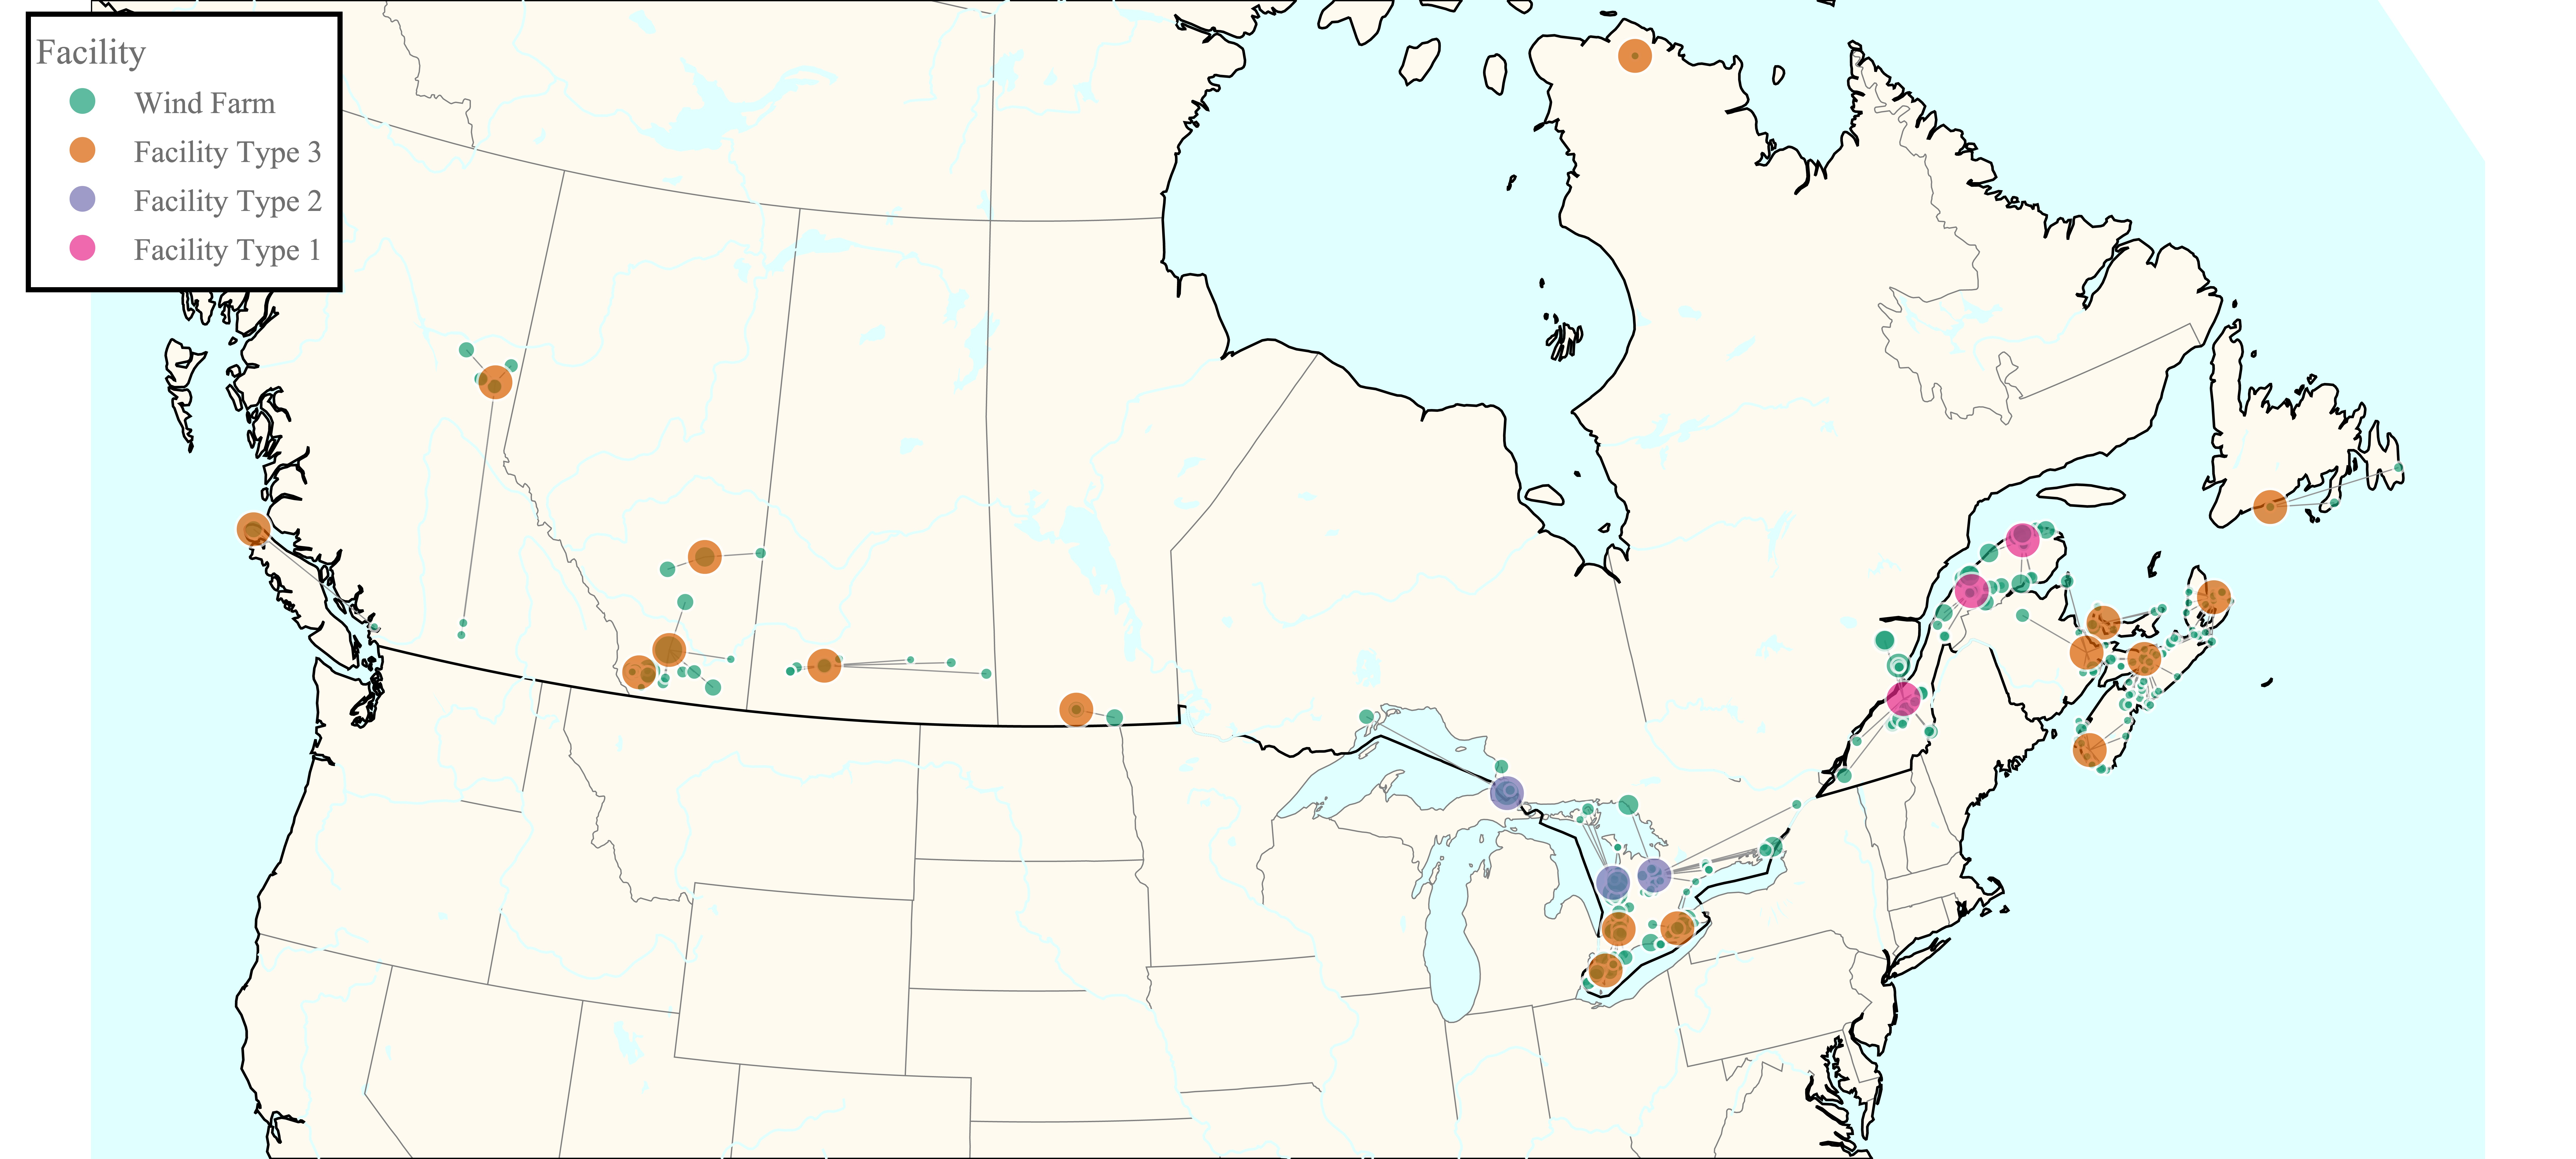
\includegraphics[width=0.9\textwidth]{graphics/fig_pbp.jpeg}
    \caption{Per Province/Territory FLP}
    \label{fig:fig_pbp}
\end{figure}

The resulting problem generated the following solution: 22 recycling facilities in Canada, 3 of Type 1, 3 of Type 2, and  16 of Type 3. The cost of delivery over 50 years is \$100 million with a total building cost of \$87.78 million. The total is approximately \$187.8 million.  

There are some limitations to this approach. First Canada is one of the largest countries by land, with unique geographic features, therefore some locations while mathematically optimal may not make practical sense. For instance, having recycling facilities in the northern territories may be invalid, because of geographic isolation for raw materials or lack of transportation. A second limitation is that we have not built in a function for additional pricing when changing transportation methods.  For instance, having a facility on the northern tip of Vancouver Island implies that the blades are loaded onto trucks then boats, which will certainly have associated costs. Therefore this location may not be as beneficial as something closer to the southern wind turbines in British Columbia, especially considering the mountainous terrain the blades would have to otherwise traverse.


%%%%%%%%%%%%%%%%
%%%FEDERAL FLP : PAN-CANADIAN OPTIMIZATION
%%%%%%%%%%%%%%%%
While we may have solved the FLP at the provincial level, the limitations of Canadian geography are a crucial consideration. Some wind farms would be better served by recycling facilities outside of their province. In fact, in the Maritimes or western Ontario, some wind farms are closer to neighboring provinces, and the cost could be reduced by sending the blades shorter distances outside of their province. Let’s assume that the federal government has nationalized this industry to meet environmental goals by 2050. In this alternate timeline, they control the subsidies and want to reduce the total amount of fixed and transportation costs. The TSP portion of this extension will not be examined as it is not an immediate legislative concern for Canada 2.0. 

In view of this problem extension, we aim to eliminate the assumption that the waste generated by a wind farm must be recycled in the same province as the wind farm. This should centralize the waste distribution and reduce the total fixed cost. Since each facility can source from a larger supply pool, they will be much closer to maximum capacity, instead of having spare capacity from the per-province mode.  

To model this assumption in our FLP, we will update our dataset by adding the wind farms from all Canadian Provinces and Canadian Territories excluding offshore wind farms, and null values briefly mentioned in the data cleaning subsection. Offshore wind farms are not considered in this FLP because the logistical requirements to recycle offshore wind farm turbines are different from land wind farms.  

We followed the same data standardization process explained in subsection \ref{subsection:dataset_description} of this paper while adding the wind farms from all Canadian Provinces to the dataset. In addition, all the assumptions, formulations and constraints developed in section \ref{section:problem_desc} are valid except for the one bounding recycling to local provinces. The optimal location results are displayed in figure \ref{fig:fig_can} below. 

\subsection{Federal FLP: Pan-Canadian Optimization}
\begin{figure} [h]
    \centering
    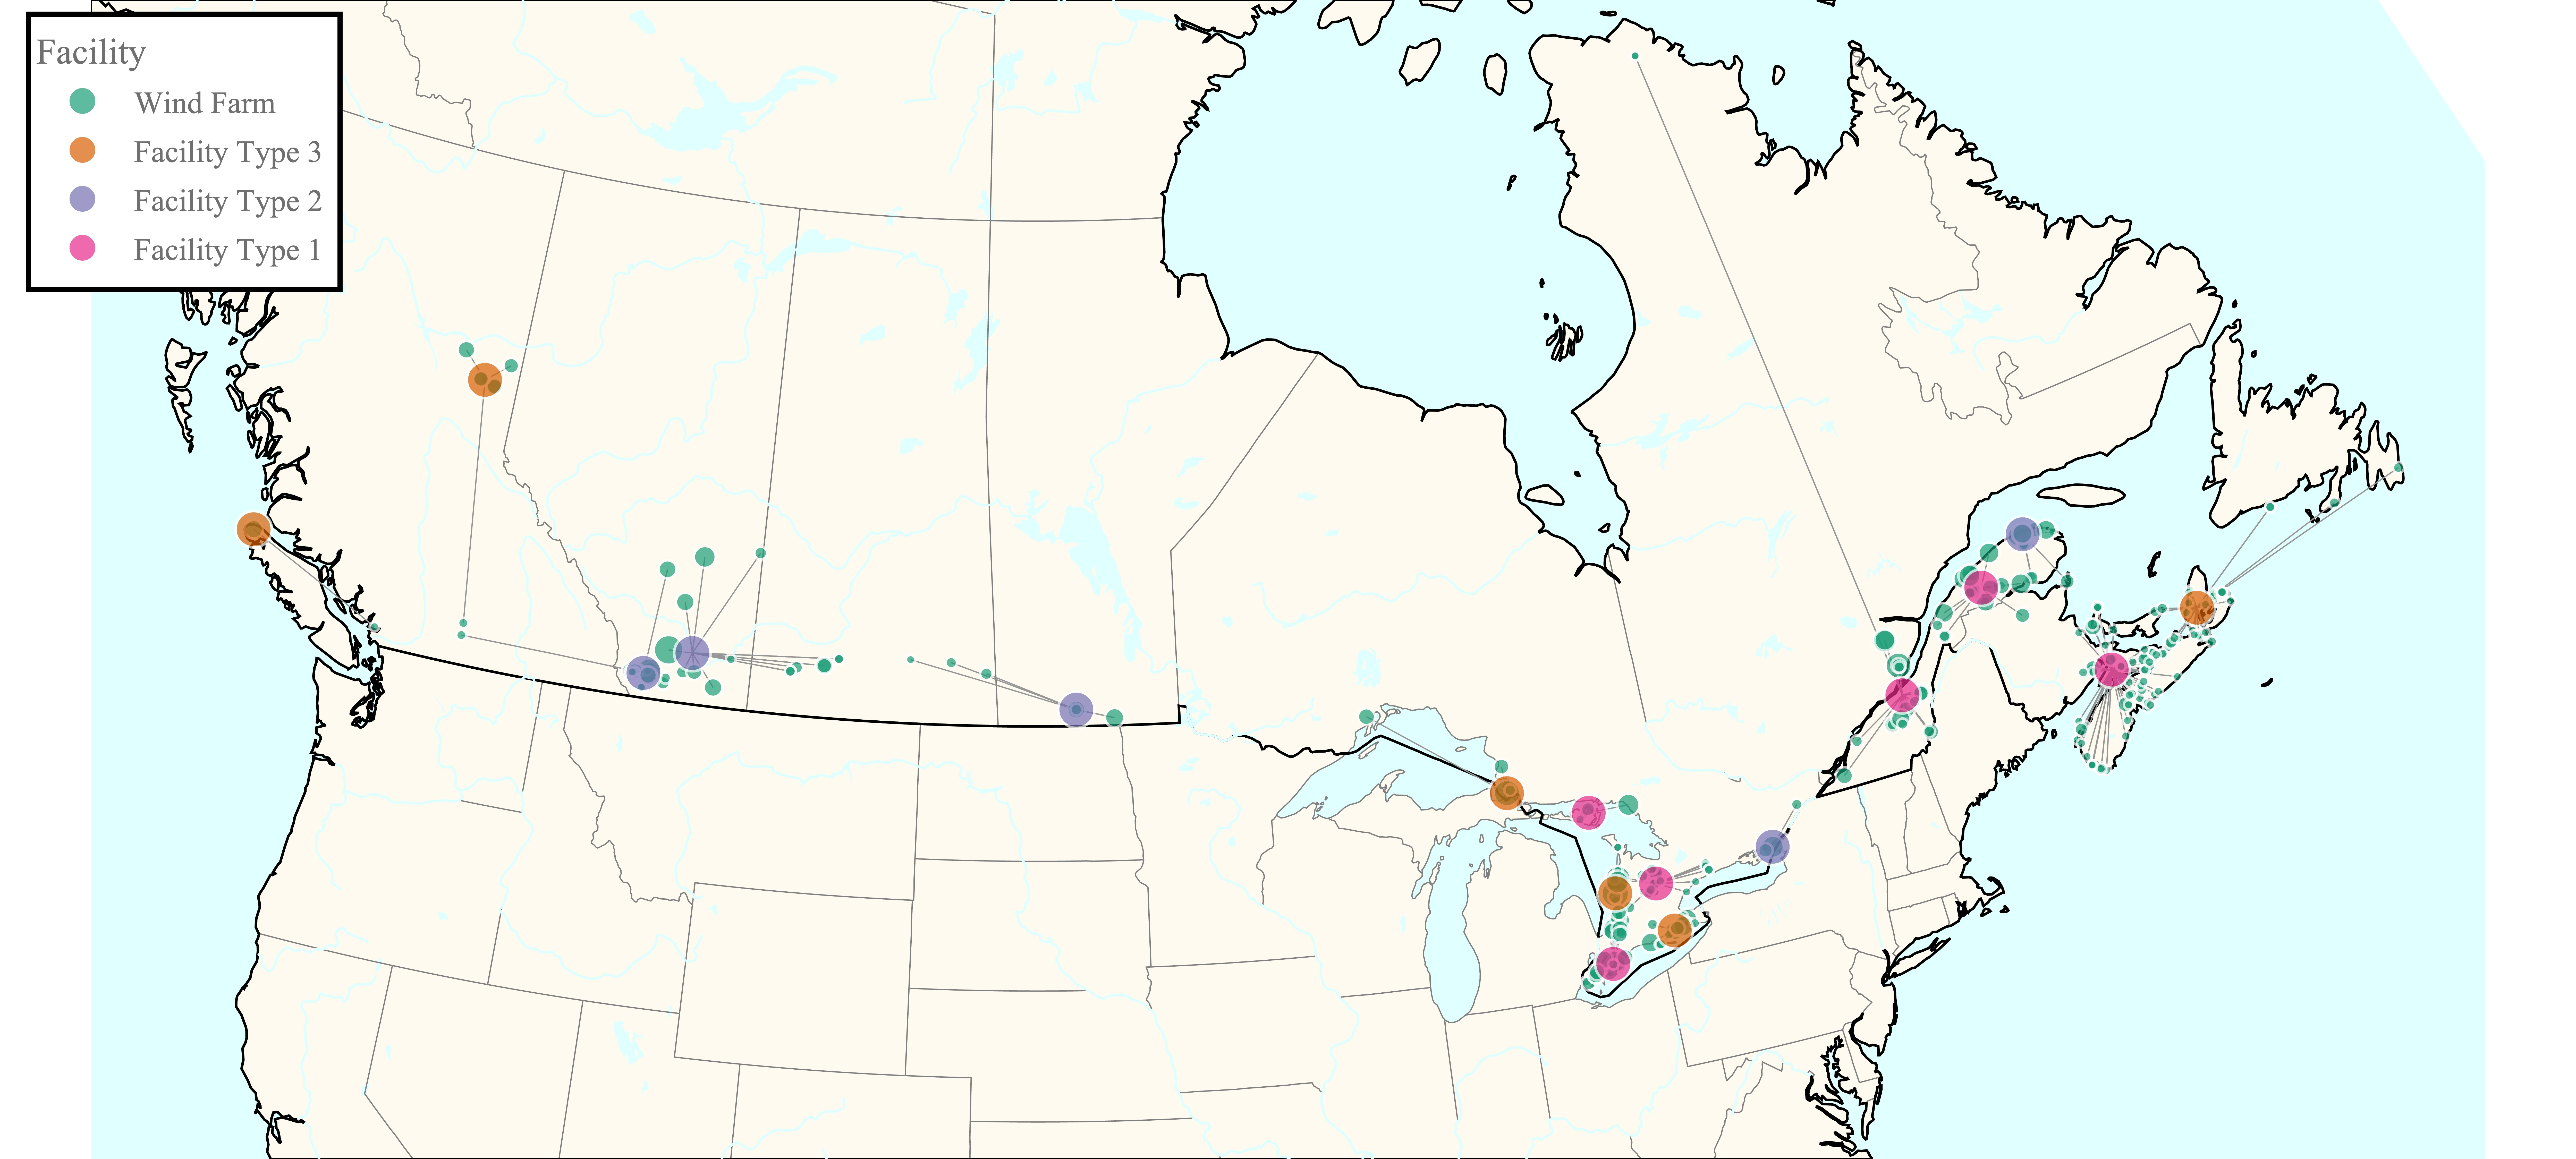
\includegraphics[width=0.9\textwidth]{graphics/fig_can.jpeg}
    \caption{Federal FLP: Pan-Canadian Optimization}
    \label{fig:fig_can}
\end{figure}

The result of the Federal FLP are the following one: 16 recycling facilities accross Canada, 6 of Type 1, 5 of Type 2, and 6 of Type 3. The cost of delivery over 50 years is \$130.33 million and the cost of building facilities is \$78.54 million. The total is therefore \$208.87 million over 50 years. This Federal FLP is far more expensive than the Per Province/Territory FLP due to delivery costs. There may be several explanations for this, however the two most likely are that the Gurobi code is limited by computational power and time. Additional optimal solutions may exist and can be solved with additional time, but we were unable to run the model for unlimited time. Furthermore, this model formulation theoretically prioritizes maximum capacity over minimum distance, as the loads from windfarms are not split and therefore the model prioritizes fixed cost savings (\$78 million vs \$87 for provincial). These limitations are best addressed with additional runtime and constraints. 



%%%%%%%%%%%%%%%%
%%%YEAR-BY-YEAR EXTENSION
%%%%%%%%%%%%%%%%
\subsection{Year-by-year extension}
With the current solution approach, we are ignoring the “lumpy” characteristic of turbine waste. Generally, all the wind blades within a wind farm must be replaced within a few years of each other. Depending on the year, there might be a significant amount of waste or none. With our current approach, there is no such “lumpy” characteristic, as we assume the supply is evenly spread over a long period. The current simplification of the facility location problem allows for efficient computational time and an approximate solution. However, the year-by-year deliveries of waste would look very different from our model and from a realistic case. 

To make the model more realistic, it is possible to extend the model by the addition of a ‘time’ index. Instead of using average annual waste, we can approximate yearly waste of wind turbines. This would allow us to better approximate real-world conditions via this formulation. By adding a $T$ set, indicating a specific year within our planning horizon we could modify our $dw$ decision variable, our demand and capacity constraints, and our objective as follows: 
%\vspace{-10pt}
\begin{equation}
    dw_{wfty} - \text{integer variable indicating how many deliveries to make from } w \text{ to } f,t \text{ in year } y
\end{equation}
\vspace{-10pt}
\begin{equation}
    \sum_{f,t} dw_{wfty} = wd_{wy} \quad \forall wy \quad \quad \text{Demand}
\end{equation}
\vspace{-10pt}
\begin{equation}
    \sum_{w} dw_{wfty} * ww_{w} \le ca_{t} * fb_{ft} \quad \forall wyt \quad \quad \text{Capacity}
\end{equation}
\vspace{-10pt}
\begin{equation}
    \sum_{wtfy} (dist_{wft} * dw_{wfty} * dc * dk) \quad \quad \text{Objective}
\end{equation}

While this addition brings the model closer to real-world conditions, expanding the problem with a time index makes the problem significantly more difficult and computationally challenging to solve. As such we would recommend splitting the problem into two phases, similarly to our current formulation. In phase 1 locating the facility locations through the average annual delivery is acceptable as the facilities have a much longer useful life than the wind farms and can reach a steady state at some point in their lifetime. Then phase 2 decides how to distribute the waste between facilities with a time index, to better represent the “lumpy” supply which may be solved as a larger instance of the problem. Additionally by having a time index, we would be able to better link the two models, by only allowing the wind blade waste to be delivered after wind blades haves been cut.

%%%%% CONCLUSION
\section*{CONCLUSION}
\addcontentsline{toc}{section}{CONCLUSION}
Managing waste remains a global challenge. The wind farm industry is growing at an increasing rate, and so are wind turbine waste, byproducts and environmental damage. We investigated the most cost-effective way of helping the province of Ontario in Canada of approaching the two key challenges this novel wind turbine recycling industry faces. A recycling facility location problem and specialized recycling vehicle routings. We modelled wind turbine recycling facility locations (fiberglass recycling facilities) in the province of Ontario over a 50-year period to minimize the facility and transportation costs. While simultaneously investigating how many specialized recycling trucks are required and what routes these trucks should take on.   

In the first stage, we used the Capacitated Multi-Facility Weber Problem to find the optimal location of recycling facilities that would minimize the total cost. Both the cost of delivering wind turbines and the fixed cost associated with the construction of a recycling facility make up the total cost. In this stage, our finding suggests that over a 50-year period, the fixed cost of building recycling facilities tends to be lower than the long-term cost of delivering wind turbines to these facilities. Therefore, somewhat counterintuitively, more facilities reduce the overall cost over 50 years. As we spread facilities throughout the province, the lower transportation costs reduce the overall cost. We pushed this location model further to expand across Canadian provinces. When comparing a provincial and a national approach, our results indicate that a provincial approach is cheaper. When each province handles recycling, each province can reduce the distance between the facility and wind farms, which is the main cost driver. Furthermore, each province can install and legislate on its own facilities to fit within its infrastructure which may be more feasible for real-world applications. A Federal Program would serve the entire country, which would maximize the facility capacity but increase transportation costs.  

In the second stage of our approach, with the Recycling Truck Service Rotation problem, the goal was to minimize the number and cost of specialized trucks that travel between wind farms to cut the discarded blades into smaller pieces for easier transportation. To reduce the complexity of the Traveling Salesperson type problem (TSP), we used a KNN clustering algorithm to determine the sub-tours. In other words, each cluster became a tour for each recycling truck. Based on movement and fixed cost, the optimal number is 3. The TSP problem will be further refined with more accurate estimates of capacity, fixed cost, transportation costs and transportation time. This second problem is an important step in long-term wind turbine recycling.  

Humans have a long-standing tendency to create problems as a direct result of solving another problem. We harness fire to create warmth, produce wonderous inventions and harness electricity only to change our environment. We harness the wind to slow the environmental damage only to create more unintended waste. Perhaps this time is different. We have the data, computational power, and an ethical business lens. We see and understand the impact of our actions and know how to fix the situation. We hope the approach to these two key challenges, location, and routing optimizations, enables a swift transition to a more sustainable, green, wind turbine industry. 

%%%%% BIBLIOGRAPHY
\newpage
\printbibliography

\end{document}  